\documentclass[]{article}
\usepackage{graphicx}
\usepackage{hyperref}
\usepackage{amsmath}
\usepackage{caption}
\usepackage{subcaption}
\usepackage[utf8]{inputenc}
\usepackage{float}

%opening
\title{Saturated Absorption Spectroscopy for the $D2$ lines of $^{87}Rb$ and $^{85}Rb$ at room temperature }
\author{Gunther T\"urk, Jonas Lehnen}

\begin{document}

\maketitle
\begin{abstract}


\end{abstract}

\newpage
\tableofcontents

\newpage
\section{Introduction}
Understanding the behaviour of excited atomic states and being able to manipulate them is a part of atomic physics. To visualize the energy transitions a spectrum has to be taken and analysed. 
This experiment about laser spectroscopy will show the problem of absorption spectroscopy (AS) regarding the resolution of the transition energy. This will be shown at the example of $^{87}Rb$ and $^{85}Rb$. The transition between $5^2S_{1/2}$ and $5^2P_{3/2}$, also called $D2$ line, will be excited with a $780nm$ laser. %%%%%%%%%%%%%% The natural linewidth
Due to Doppler broadening an atom can be excited in a wider range of energy, thereby it is not possible to resolve the hyperfine structure in this case. The application of saturated absorption spectroscopy (SAS) will improve the spectrum to shown the exact transitions within the Doppler broadening.

\newpage
\section{Theory}
\subsection{Absorption spectroscopy}
The transmitted intensity of light after the transition through matter can be described with the Lambert Beer law. The transmission $T$ depends on the materials length $L$ and the absorption coefficient $\alpha$ which is depending on the resonance frequency $\omega_0$ of the individual atomic transitions as well the natural linewidth $\Gamma$ of this transition.

\begin{equation}
T(\omega)\approx 1-\alpha(\omega)L \:,\: \alpha(\omega)= \alpha(\omega_0)\frac{\Gamma/2\pi}{(\omega-\omega_0)^2 + (\Gamma/2\pi)^2}
\end{equation}

This results in a valley in the intensity for each $\omega_0$ the laser stimulates, due to the maximum in absorption. Each minimum should be formed like a Lorentzian, due to the prportionality in $\alpha$. For fitting this curve is not useful, because a standard derivation is not properly defined. 

\subsection{Doppler broadening}
The natural linewidth $\Gamma$ describes for which frequency around $\omega_0$ the transition can be driven. This is equal to the full width at half of the maximum (FWHM) $\delta\omega_{Natural} = \Gamma$. For a Gaussian the relation $FWHM = 2 \sqrt{2ln(2)} \sigma$ is used.

Now the Doppler effect is able to increase this range of frequencies depending on the atoms velocities relative to the incoming photons. Thereby their frequency is increased when moving towards each other and decreased in the case of moving in the same direction. For the first case, this mean a photon with $\omega < \omega_0$ can already excite the atom. And thereby the range of exciting frequencies is increased. This is described by \autoref{dopplershift} where $\vec{k}$ and $\vec{v}$ are the wave vector of the photon and the velocity of the atom.

\begin{equation}
\omega  = \omega_0 + \vec{k}\vec{v} = \omega_0 \left(1+\frac{v_{||}}{c} \right)\:,\: c = \omega_0\cdot |\vec{k}|
\label{eq:dopplershift}
\end{equation}

For a system in thermal equilibrium the velocity distribution for $v_{||}$, in direction of the photons, is given by the the Maxwell-Boltzmann distribution for N particles. 

\begin{equation}
n(v_{||})dv_{||} = \frac{N}{v_W \cdot \sqrt{\pi}} exp\left[ - \frac{v_{||}^2}{v_W^2} \right] dv_{||} \:,\: v_W= \sqrt{\frac{2k_BT}{m}}
\end{equation}

This includes the mass of the atoms m as well as the temperature T of the whole system. The transmitted intensity is directly proportional to $n(v_{||}) dv_{||}$, because this returns the atoms which are able to drive the excitation. Rewriting $v_{||}$ with \autoref{eq:dopplershift} we end up with a Gaussian for each $\omega_0$ in our spectrum of the Doppler broadening.

\begin{equation}
I(\omega)=I(\omega_0)\ exp\left[ - \frac{(\omega-\omega_0)^2}{\omega_0v_{||}\ / c}\right] \:,\: \delta\omega_{Doppler} = 2 \sqrt{ln(2)} \cdot \omega_0\frac{v_W}{c}
\label{eq:gauss}
\end{equation}

For room temperature $T=300K$ this results in $\delta\omega_{D} \approx 3201\ MHz$. Compared to the usual hyperfine transitions for the excited state in \autoref{fig:Rb_hyperfine}, this value is too high to resolve those transitions. Therefore a different approach has to be made.

\subsection{Saturated absorption spectroscopy}



\newpage
\section{Experimental set-up}
\begin{figure}[H]
\centering
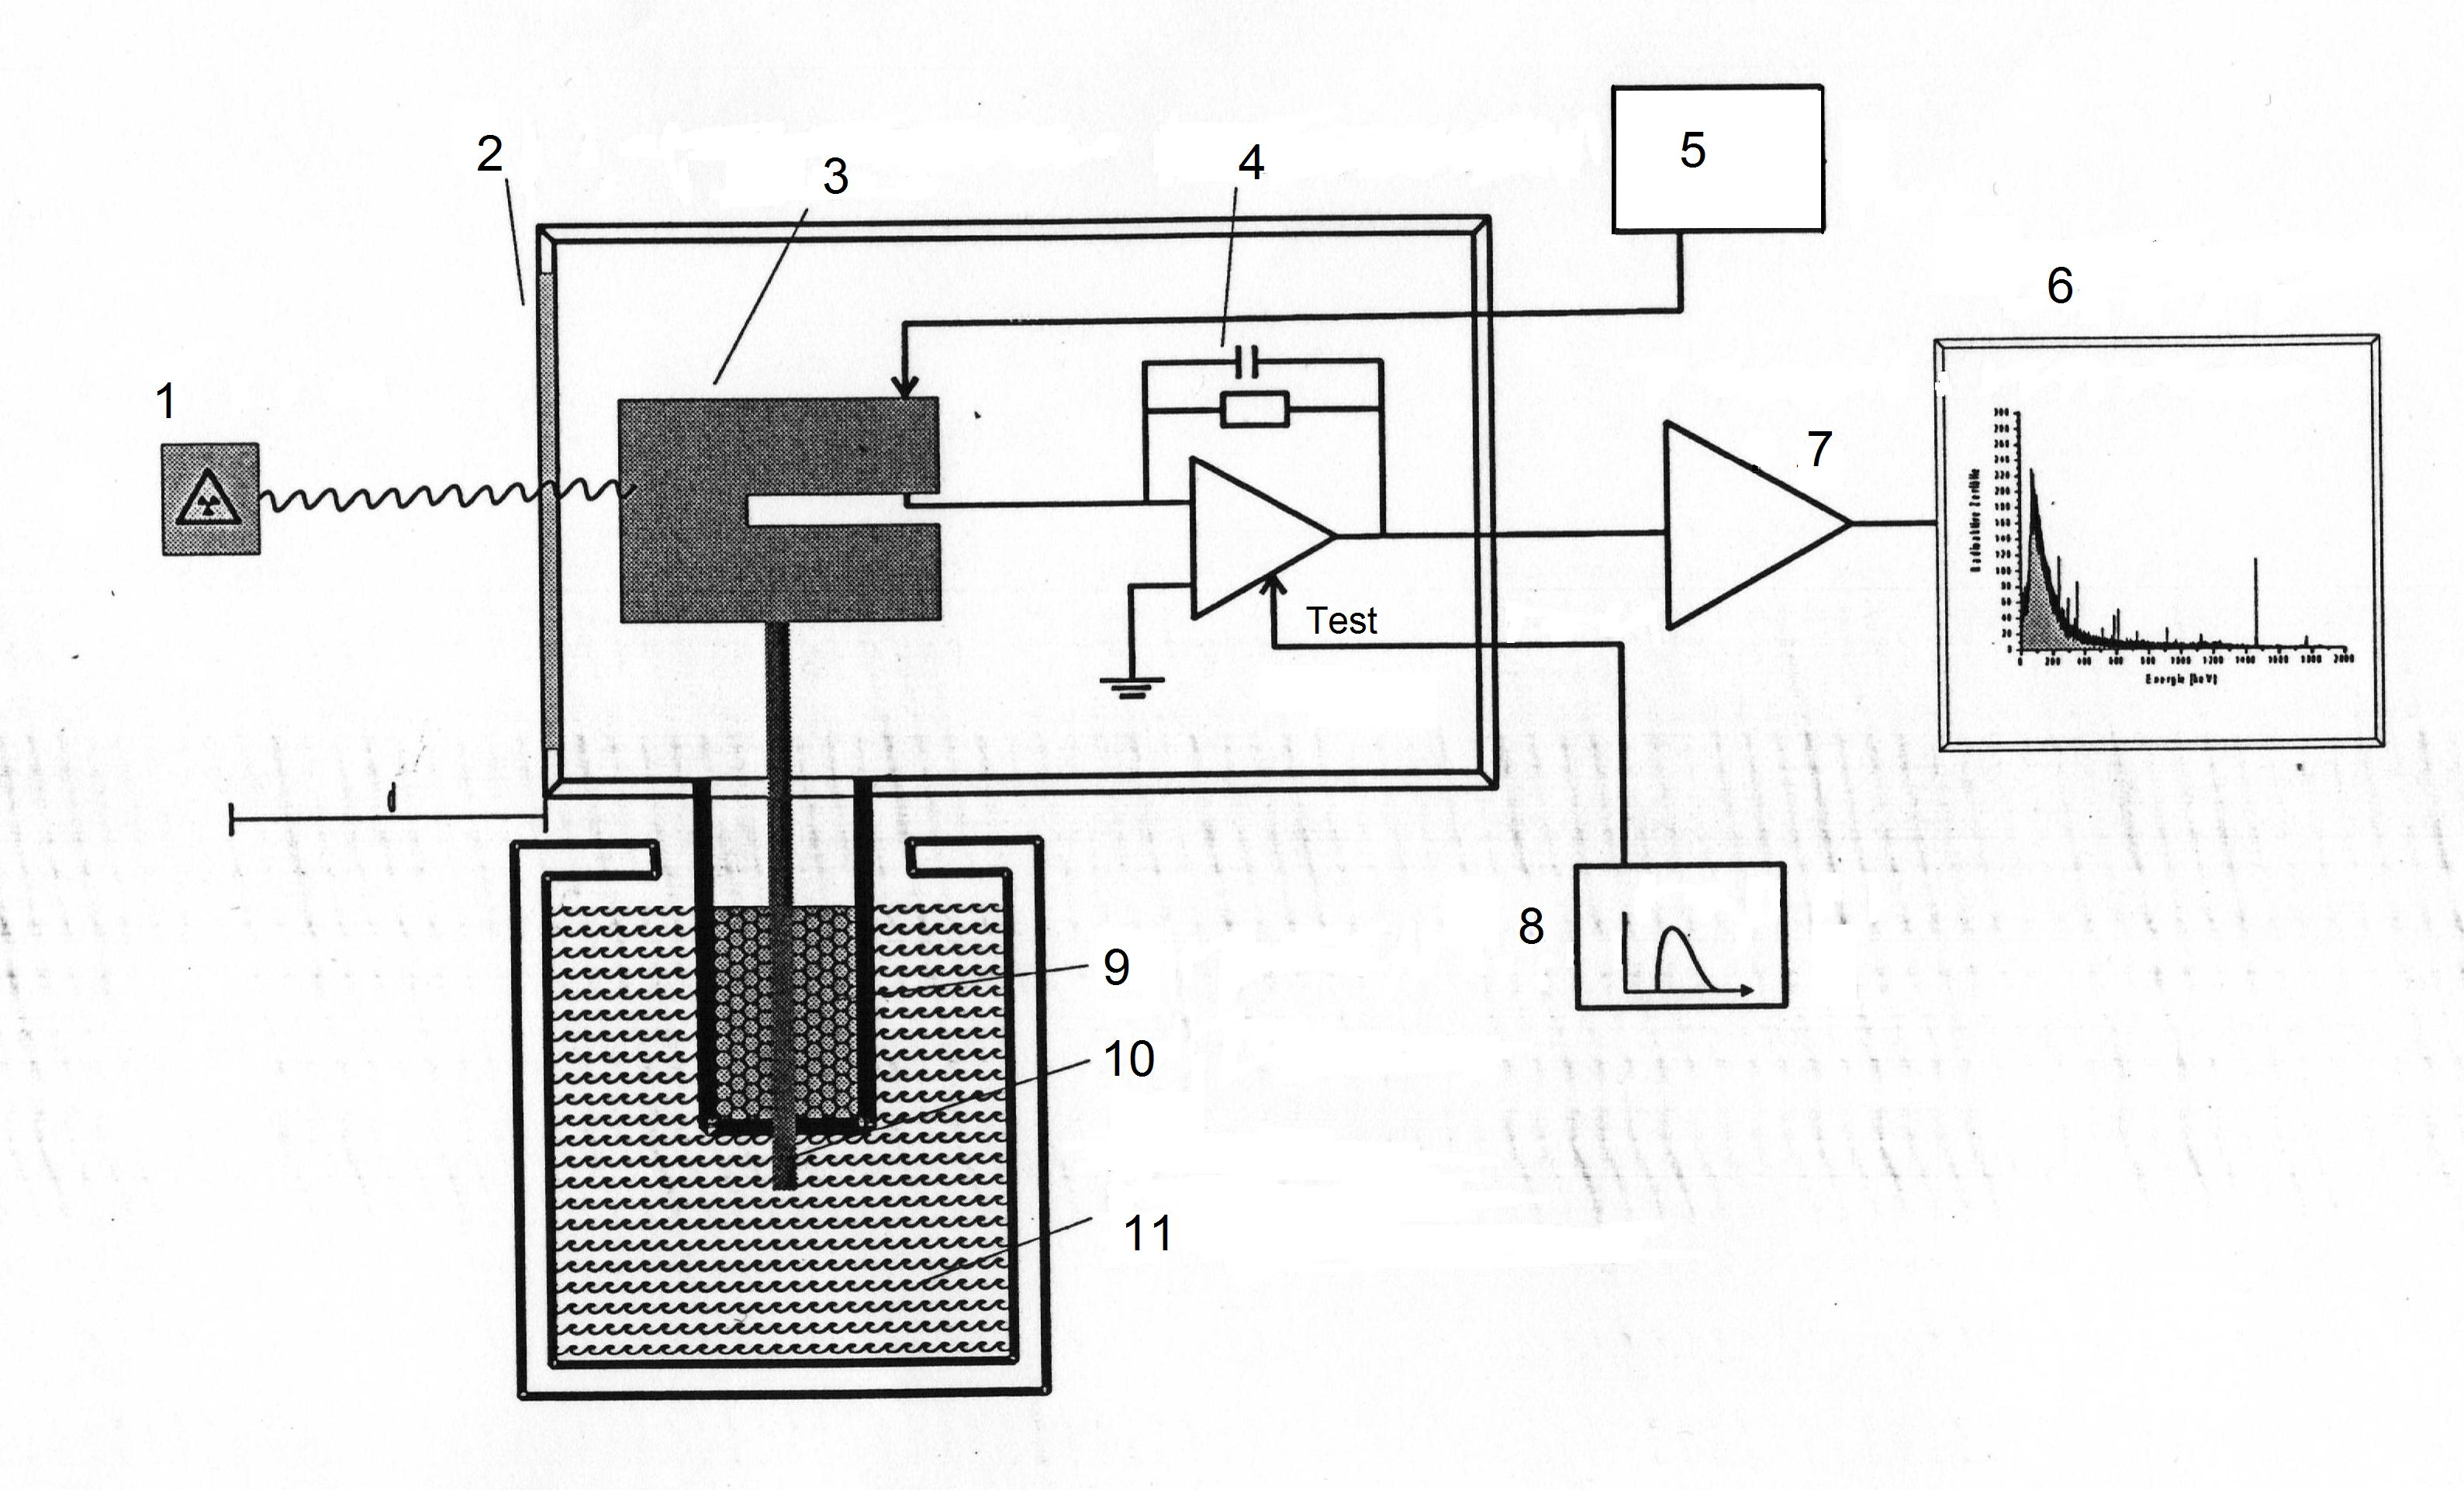
\includegraphics[width=1\textwidth]{Plots/Setup.png}
\caption{Schematics of the experimental set-up used.}
\end{figure}

For this experiment a rubidium gas cell of the isotopes $^{85}Rb$ and $^{87}Rb$ with an ratio of $72.2 : 27.8$ is used. The wavelength of the laser was set on $780.24nm$.

%%%%% ramp gen fährt freq durch, aufsteigend -> labelling of the peaks


\newpage
\section{Analysis}
\subsection{Spectrum}
\begin{figure}[H]
\centering
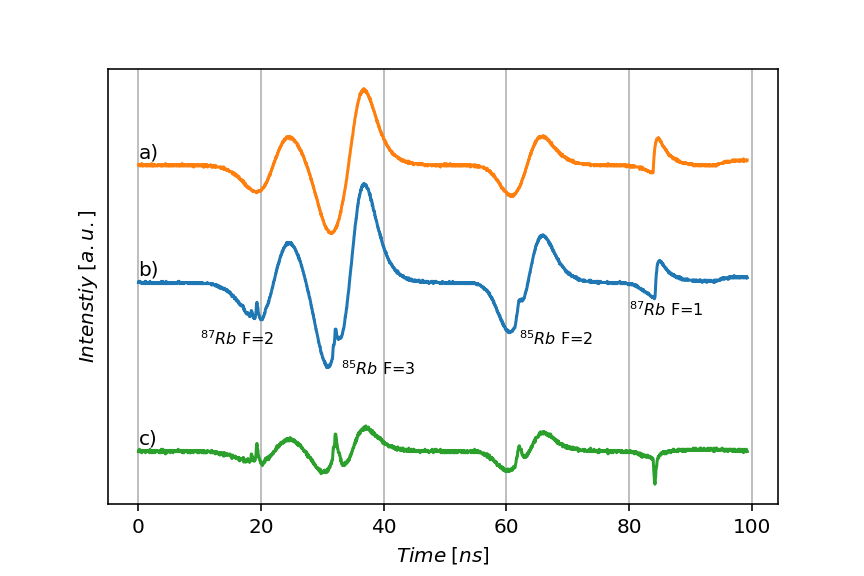
\includegraphics[width=.8\textwidth]{Plots/Diff_Signal.png}
\caption{Spectrum of the rubidium gas cell. a) AS, b) SAS, c) Difference signal}
\label{fig:signals}
\end{figure}

As shown in \autoref{fig:signals} the difference between the spectra of the different methodes are grave. As expected a) shows no hyperfine transitions due to insufficent resolution. For b) those are now clearly visible and will be used to identify the transitions in the following chapters. They are already labelled according to the transitions shown in \ref{fig:Rb_hyperfine}.
The difference signal c) should only show the peaks of the hyperfine structure.

\subsection{Calibration}
\begin{figure}[H]
\centering
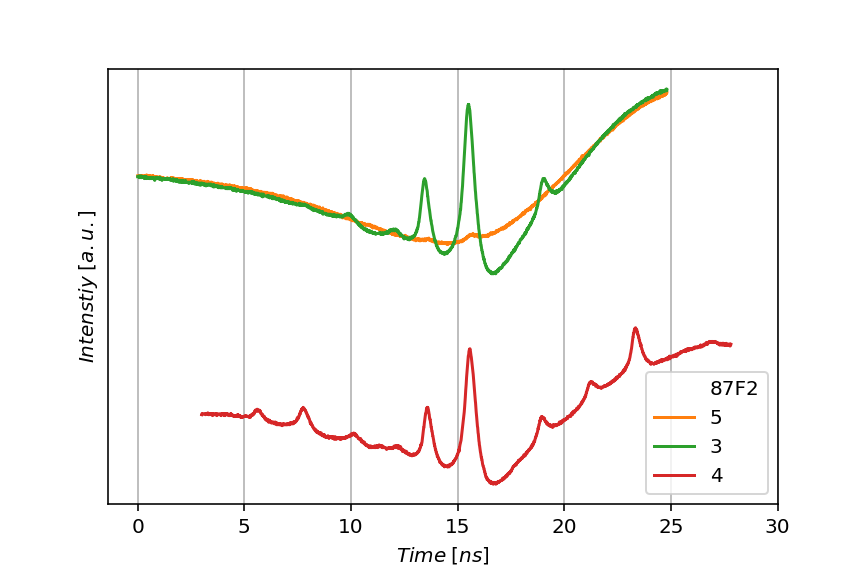
\includegraphics[width=.8\textwidth]{Plots/Calibration_Second_All.png}
\caption{Graphic of the difference between AS and SAS. The hyperfine structure transitions are now visible. In red the SAS while an additional signal generator is on to create the sidebands for calibration purposes.}
\label{fig:all}
\end{figure}

The measurement data taken from the oscilloscope consists of intensities and the time. The orange line for absorption spectroscopy and the green one for saturated AS shifted on top are showing the difference between the methodes.
To determine at which energy a peak is it is necessary to convert the time into an energy or according frequency scale. This is done with the red curve in \autoref{fig:all}. An additional signal generator creates the sidebands in a set frequency distance of $\omega_{shift}=600MHZ$. These sidebands are the difference between green and red curve. They are echoes of the peaks already seen but shifted by $\omega_{shift}/2$ in both directions. Determination of the expected value of each peak in the red curve leads to the conversion rule from time to energy. 

\autoref{fig:calibration} is created by subtracting the AS spectrum from the red curve to increase the visibility of the peaks for better results while fitting them. The fits are Gaussian due to \autoref{eq:gauss} with an error given by the standard derivation $\sigma$. Gaussian function with $\mu$ as expected value:

\begin{equation}
G(x) = A \cdot exp\left( -\frac{(x-\mu)^2}{2\sigma^2} \right)
\end{equation}

\begin{figure}[H]
\centering
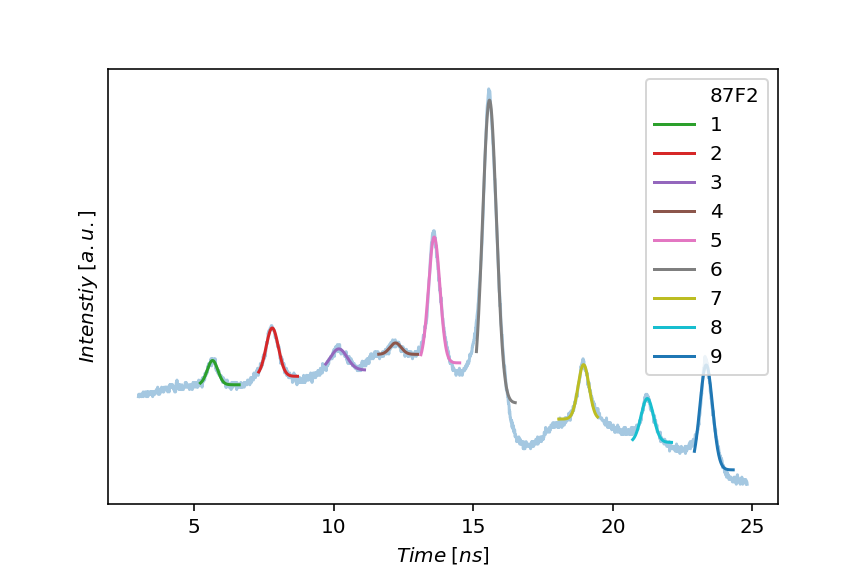
\includegraphics[width=.8\textwidth]{Plots/Calibration_Second_Real.png}
\caption{Saturated absorption spectroscopy with sidebands subtracted with the curve for AS. This improves the visibility of the individual peak. They are already named as explained later.}
\label{fig:calibration}
\end{figure}

%%%%% The naming of the peaks will be discussed in \ref asdas



\begin{table}[H]
\centering
\begin{tabular}{c|c|c}

Peak 1 & Peak 2 & Difference [ns] \\ \hline\hline
SB CO13 left & CO13 & $7.94 \pm 0.28$ \\
CO13 & SB CO13 right & $7.63 \pm 0.31$ \\ \hline 
SB CO23 left & CO23  & $7.78 \pm 0.34$ \\
CO23 & SB CO23 right & $7.75 \pm 0.36$

\end{tabular}
\caption{Time difference between expected values of the peaks as labelled in \autoref{fig:calibration}. The error is given by: $\sqrt{\sigma_1^2 + \sigma_2^2}$.}
\label{tab:calc}
\end{table}

By dividing the equivalent $300MHz$ per time difference shown in\autoref{tab:calc} with the average value of $7.78 \pm 0.32$ results in the following conversion rule.
\begin{equation}
1ns = 38.56 \pm 1.59 \ MHz
\label{eq:conversion rule}
\end{equation}


\newpage
\subsection{Rubidium 87, F=2}
\begin{figure}[H]
\centering
\begin{subfigure}{.7\textwidth}
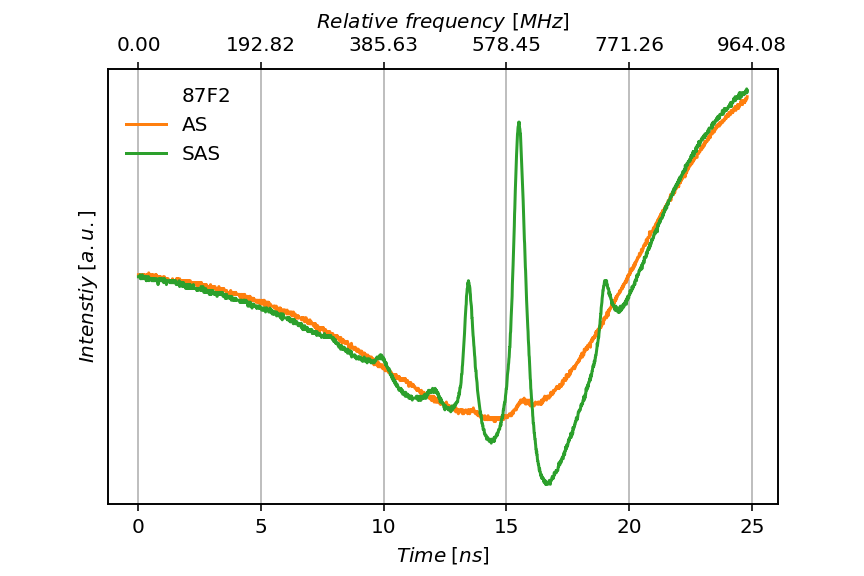
\includegraphics[width=\linewidth]{Plots/87F2_Both.png}
\end{subfigure}

\begin{subfigure}[c]{.7\textwidth}
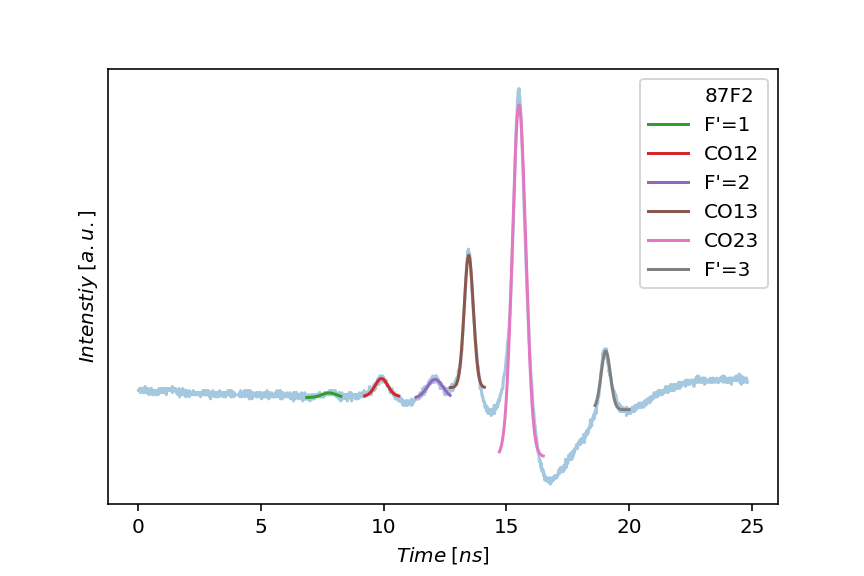
\includegraphics[width=\linewidth]{Plots/87F2_Diff.png}
\end{subfigure}
\caption{Measured signals on top and difference signal with Gaussian fits for each visible peak underneath.}
\label{fig: 87F2}
\end{figure}

%%% tabel with postional values

\newpage
\subsection{Rubidium 85, F=3}
\newpage
\subsection{Rubidium 85, F=2}
\newpage
\subsection{Rubidium 87, F=1}

\newpage
\section{Discussion}


\newpage
\section{Appendix}
\subsection{Rubidiums hyperfine structure}
\begin{figure}[H]
\centering
\begin{subfigure}{.8\textwidth}
\centering
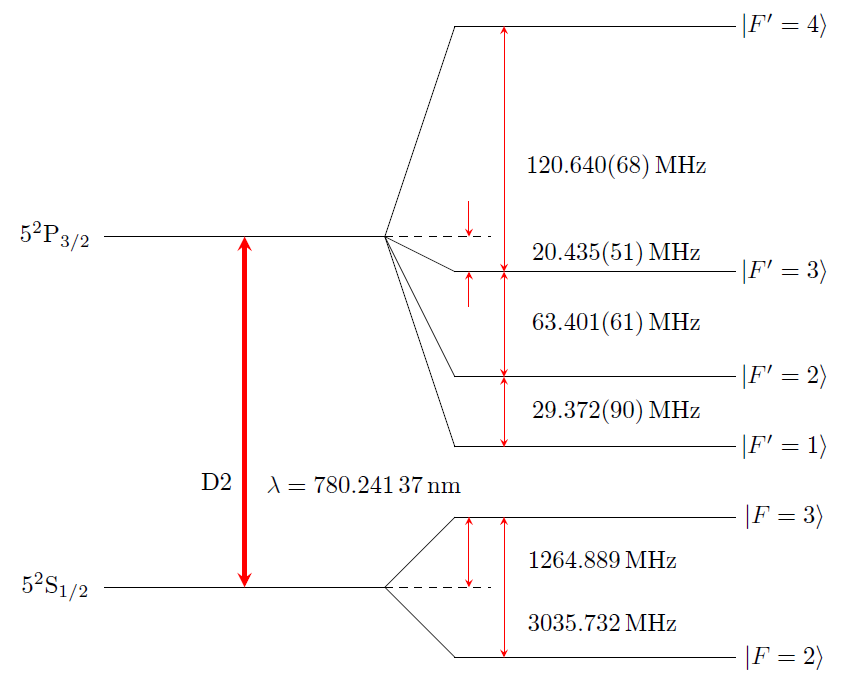
\includegraphics[width=1\textwidth]{Plots/Level85.png}
\caption{Hyperfine structure of Rubidium 85 \cite{steck85} }
\end{subfigure}

\begin{subfigure}{.8\textwidth}
\centering
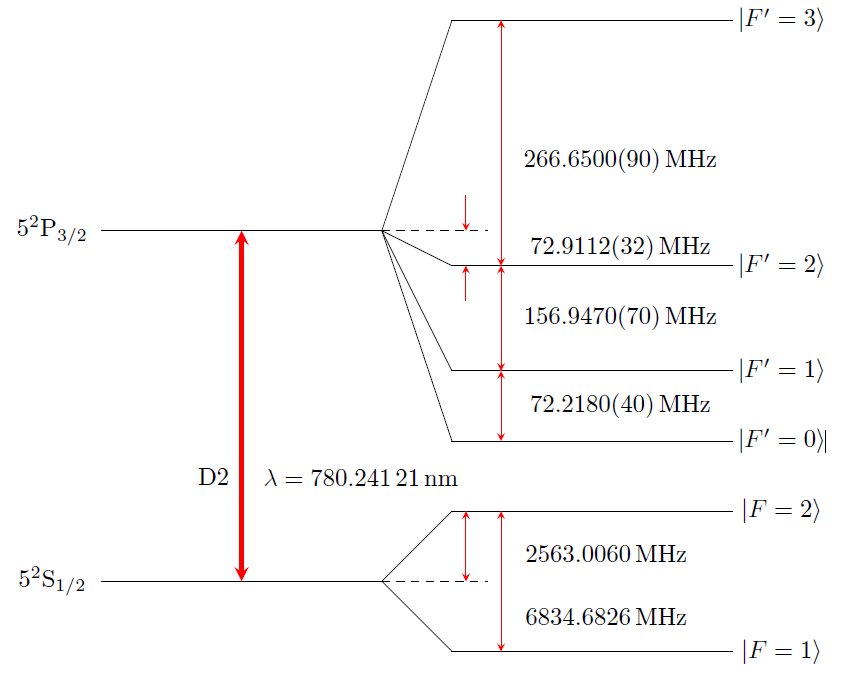
\includegraphics[width=1\textwidth]{Plots/Level87.png}
\caption{Hyperfine structure of Rubidium 87 \cite{steck87}}
\end{subfigure}

\caption{Hyperfine structure of both used rubidium isotopes.}
\label{fig:Rb_hyperfine}
\end{figure}

\newpage
\begin{thebibliography}{}
\bibitem[Steck85]{steck85} Rubidium 85 D Line Data, Daniel Adam Steck, University of Oregon

\bibitem[Steck87]{steck87} Rubidium 87 D Line Data, Daniel Adam Steck, University of Oregon


\end{thebibliography}
\end{document}

